\begin{problem}{전생했더니 슬라임 연구자였던 건에 대하여 (Easy)}{standard input}{standard output}

안녕? 내 이름은 ntopia!

나는 원래 지구에 살고있던 평범한 20대 청년이었어. 어느날 길을 걷다가 괴한의 칼에 찔려
죽어버렸어. 그런데 이게 무슨 일이람! 정신을 차려보니 이세계에 떨어져버렸지 뭐야.
여기에서 나는 슬라임을 전문으로 연구하는 슬라임 연구자가 되어버린 것 같아.
나는 지금 아주 중요한 연구를 진행하고 있어. 이 연구가 성공하면 나는 내가 살던 세계로
돌아갈 수 있게 될거야. 이 연구를 도와주지 않겠니?

이 곳의 슬라임은 모두 슬라임 에너지라는 것을 갖고 있고 그 양은 2 이상의 자연수로 표현돼.
나는 슬라임을 분할했을 때 슬라임 에너지가 어떻게 변화하는지에 대해 연구하고 있어.

슬라임 분할 과정은 1마리를 분할해서 2마리를 만들어내는 식으로 이루어져.
$K$만큼의 슬라임 에너지를 갖고 있는 슬라임이 있었다고 해보자. 이 슬라임을 적절히 분할하면
$A$만큼의 에너지를 갖고 있는 슬라임과
$B$만큼의 에너지를 갖고 있는 슬라임을 만들 수 있고 ($A$, $B$는 2 이상의 자연수),
항상 $K = A * B$ 를 만족해.
이렇게 분할하다보면 언젠가는 분할이 되지 않는 슬라임도 생기겠지?

그리고 슬라임 분할 기술이 아직 완벽하지 않아서 슬라임을 분할할 때마다
흠집이 하나씩 생기게 돼. 구체적으로, 흠집이 $T$개인 슬라임을 분할하면
흠집이 $T+1$개인 슬라임 2마리가 생기는 것이지.

\begin{center}
  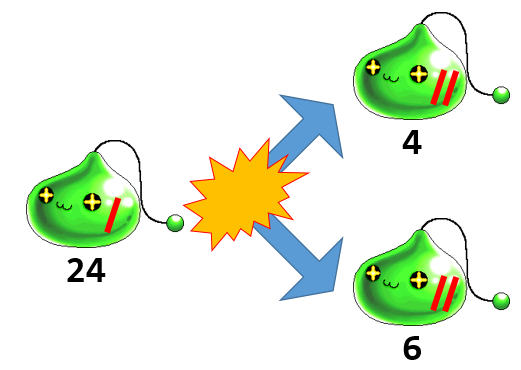
\includegraphics[width=1\textwidth]{slime_divide.png}
\end{center}

나에겐 지금 슬라임 에너지가 $K$이고 흠집이 하나도 없는 슬라임이 있어.
이 슬라임을 분할하고 또 분할해서 분할이 가능한 슬라임이 존재하지 않을 때 까지 마구마구 분할해야해.
그렇게 다 분할하고나면 마지막에 남은 슬라임들에 흠집이 적당히 생겼겠지?
(물론 생기지 않았을 수도 있어)
그 슬라임들 중에서 흠집이 제일 많이 생긴 녀석의 흠집의 개수가 최소가 되도록
분할을 적절히 수행하는 것이 내 연구의 목표야.

내 연구를 도와줘! 부탁이야!!

\InputFile
첫 번째 줄에 처음 주어진 슬라임의 에너지 $K$ ($2 \le K \le 100,000$) 가 주어진다.

\OutputFile
슬라임을 끝까지 분할했을 때, 가장 많이 생긴 흠집의 개수의 최소값을 출력한다.

\Example

\begin{example}
\exmp{10}{1}%
\exmp{3}{0}%
\exmp{24}{2}%
\end{example}

\Notes
처음에 에너지가 24이고 흠집이 없는 슬라임이 있다.
이 슬라임을 에너지가 4인 슬라임과 6인 슬라임으로 분할할 수 있고 각각은 흠집이 1개가 된다.

에너지가 4이고 흠집이 1개인 슬라임은 에너지가 2이고 흠집이 2개인 슬라임 2마리로 분할할 수 있다.

에너지가 6이고 흠집이 1개인 슬라임은 에너지가 2이고 흠집이 2개, 에너지가 3이고 흠집이 2개인 슬라임으로 분할할 수 있다.

이렇게 분할하고 나면 더이상 분할이 가능한 슬라임이 존재하지 않게 된다.

이 때 가장 많이 생긴 흠집의 개수는 2개이다. 이보다 더 적게 되도록 분할하는 방법은 존재하지 않는다.

\end{problem}
